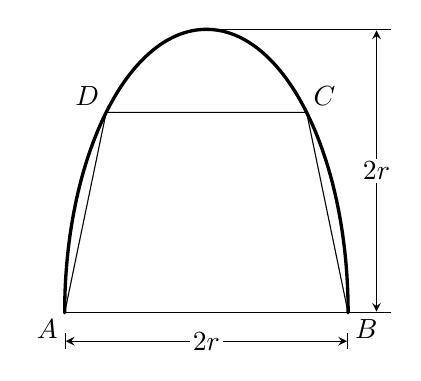
\begin{tikzpicture}[>=stealth, scale=0.9, line cap=round, line join=round]
  % Ellipse arc: x = 2*cos(t), y = 4*sin(t) for t from 0 to 180 degrees
  \draw[very thick] (2, 0) arc[start angle=0, end angle=180, x radius=2, y radius=4];

  % Bottom edge AB
  \coordinate (A) at (-2, 0);
  \coordinate (B) at (2, 0);
  \draw (A) -- (B);

  % Inscribed trapezoid ABCD
  % at t = 45 deg, x = 2*cos(45) = 1.414, y = 4*sin(45) = 2.828
  \coordinate (C) at (1.414, 2.828);
  \coordinate (D) at (-1.414, 2.828);

  \draw (A) -- (D) -- (C) -- (B);

  % Vertex labels
  \node[below left=-1pt] at (A) {$A$};
  \node[below right=-1pt] at (B) {$B$};
  \node[above left=-1pt] at (D) {$D$};
  \node[above right=-1pt] at (C) {$C$};

  % Dimension line for AB (width 2r)
  \draw[|<->|] (-2, -0.4) -- (2, -0.4) node[midway, fill=white, inner sep=1pt] {$2r$};

  % Dimension line for height (2r)
  \draw (0, 4) -- (2.6, 4);
  \draw (2, 0) -- (2.6, 0);
  \draw[|<->|] (2.4, 0) -- (2.4, 4) node[midway, fill=white, inner sep=1pt] {$2r$};
\end{tikzpicture}
